\chapter{Conclusiones y trabajos futuros}

Se desarrolló la herramienta \emph{VMT} para la realización de espectáculos de \emph{video mapping} que implementa un enfoque novedoso permitiendo la utilización de modelos tridimensionales para representar las superficies a proyectar y posibilitando la aplicación de efectos directamente sobre ellos. Cuenta con una interfaz de usuario interactiva donde es posible visualizar los efectos en tiempo real a medida que se van diseñando.
Se lograron identificar etapas claramente diferenciadas del proceso de creación de un espectáculo, lo cual fue muy útil para delinear requerimientos específicos para la implementación de \emph{VMT}. 
En las entrevistas que se mantuvieron con los \emph{VJs} surgió como un problema común a resolver el de las costuras en áreas donde se solapan las proyecciones en espectáculos que utilizan más de un proyector. Mediante el soporte de múltiples proyectores \emph{VMT} evita este problema al tener control sobre lo que proyecta cada uno de los proyectores y permite definir en qué proyector se visualizan cada uno de los objetos y sus efectos asociados. Más en general, el manejo de múltiples proyectores distribuidos posibilita la creación de distintos esquemas de proyección soportando áreas amplias y disjuntas e incluso mapeos en 360 grados.

\paragraph{Obtención automática de la geometría}

Se logró resolver parcialmente el problema de reconstrucción automática de la escena a mapear mediante la implementación de una aplicación que toma una nube de puntos ya capturada, la procesa y genera un objeto tridimensional en un formato soportado por \emph{VMT}.
Se trabajó en el estudio de las técnicas y componentes existentes para la reconstrucción tridimensional de la escena, principalmente mediante la utilización del método de luz estructurada, en donde se experimentaron varios problemas, la mayoría de ellos en la etapa de calibración del sistema cámara-proyector. 
Se logró realizar exitosamente una prueba de concepto del método de escaneo de Kyle McDonald  Three-Phase shift.
% (poner imagen de mi cara)
Si bien este método logra obtener una representación tridimensional, tiene limitantes en cuanto a que las superficies a escanear deben ser continuas. Es por esta razón que fue descartado ya que escenas normalmente utilizadas en espectáculos de video mapping utilizan por lo general geometría discontinua.
Si bien existen otros métodos de escaneo con luz estructurada que se adaptan mejor a superficies discontinuas, no existían prototipos ya desarrollados para realizar pruebas de concepto y se consideró fuera del alcance del proyecto.

Durante el transcurso del proyecto surgió el dispositivo Kinect para el escaneo en tiempo real de objetos utilizando una implementación de luz estructurada. Con la liberación de su kit de desarrollo se incentivó su uso a desarrolladores de todo el mundo y para una variedad de propósitos. Esto motivó a enfocar el alcance en cuanto a la obtención de geometría en el procesamiento de la nube de puntos, independiente de cómo estos puntos se obtienen y finalmente abandonar el estudio de escáneres de bajo costo a incluir como parte del proyecto, ya que Kinect logra buenos resultados y es accesible en términos de costos.

\paragraph{Espectáculos en vivo}

Se realizaron dos espectáculos en vivo con la herramienta \emph{VMT} en una versión alfa: el evento de cierre de Ingeniería de Muestra año 2010\footnote{\url{http://www.fing.edu.uy/eventos/ingenieria_demuestra/2010/index.html}} y una exposición durante la noche de fallos de fin de curso de la Facultad de Arquitectura de la Universidad de la República.
\begin{figure}[H]
  \centering
    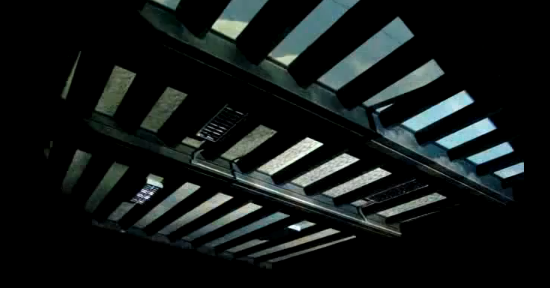
\includegraphics[width=0.7\textwidth]{./Cap7_conclusiones/ingMuestra1.png}
  \caption[Ingeniería de muestra 2010, \emph{quads} se iluminan al ritmo del audio.]{Ingeniería de muestra 2010, \emph{quads} se iluminan al ritmo del audio.}
  \label{fig:ingMuestra1}
\end{figure}
\begin{figure}[H]
  \centering
    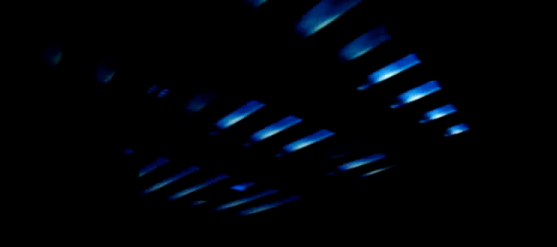
\includegraphics[width=0.7\textwidth]{./Cap7_conclusiones/ingMuestra2.png}
  \caption[Ingeniería de muestra 2010, videos en cada \emph{quad}.]{Ingeniería de muestra 2010, videos en cada \emph{quad}.}
  \label{fig:ingMuestra2}
\end{figure}

\begin{figure}[H]
  \centering
    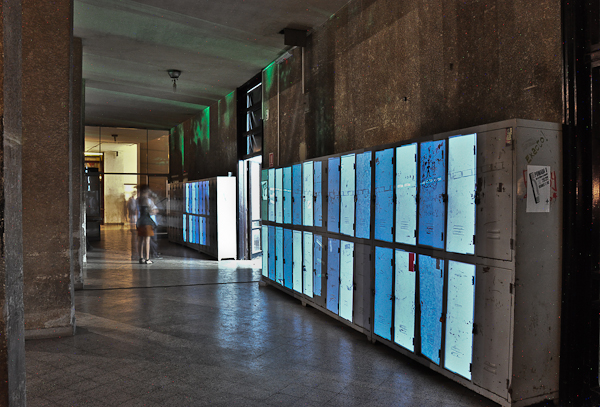
\includegraphics[width=0.7\textwidth]{./Cap7_conclusiones/Arqui1.jpg}
  \caption[Fallos fin de curso Fac.Arquitectura, casilleros iluminados.]{Fallos fin de curso Fac.Arquitectura, casilleros iluminados.}
  \label{fig:Arquitectura1}
\end{figure}

\begin{figure}[H]
  \centering
    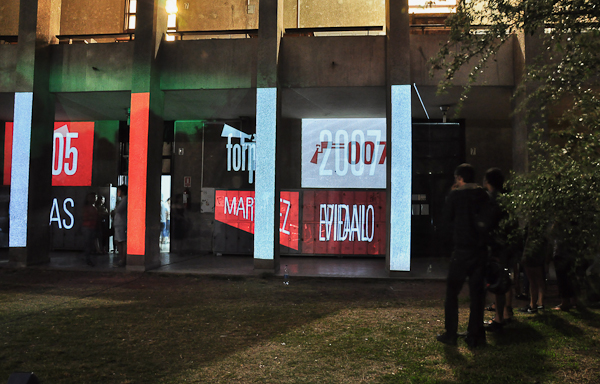
\includegraphics[width=0.7\textwidth]{./Cap7_conclusiones/Arqui2.jpg}
  \caption[Fallos fin de curso Fac.Arquitectura, casilleros y columnas iluminados.]{Fallos fin de curso Fac.Arquitectura, casilleros y columnas iluminados.}
  \label{fig:Arquitectura2}
\end{figure}

\begin{figure}[H]
  \centering
    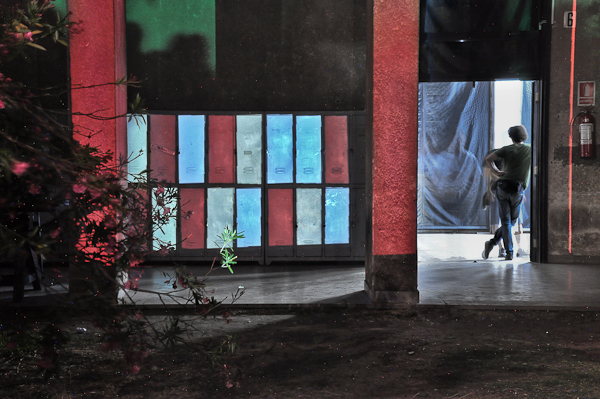
\includegraphics[width=0.7\textwidth]{./Cap7_conclusiones/Arqui3.jpg}
  \caption[Fallos fin de curso Fac.Arquitectura, casilleros y columnas cambiando de colores.]{Fallos fin de curso Fac.Arquitectura, casilleros y columnas cambiando de colores.}
  \label{fig:Arquitectura3}
\end{figure}

Durante la preparación y ejecución de los mismos se adquirió un conocimiento más profundo de qué es lo que se necesita para llevar adelante un espectáculo de estas características, lo que ayudó a definir las funcionalidades básicas que la aplicación debía cubrir. También se experimentó la importancia de la robustez y tolerancia a fallos que debe tener una aplicación que tiene como propósito la ejecución de espectáculos en vivo.
Desde el punto de vista funcional, se identificaron varios aspectos de la aplicación en las que se debía trabajar para mejorarlos, como ser el agregado de un mismo evento en varios momentos en la línea de tiempo, la agrupación de \emph{quads} para aplicarles el mismo efecto especificándolo una única vez, la ejecución del espectáculo a partir de un instante dado de la línea de tiempo, todo lo anterior accesible mediante una interfaz gráfica de usuario que adopte criterios encontrados en aplicaciones orientadas al diseño en términos generales.
En las instancias iniciales del desarrollo de la aplicación, se había decididido distribuir los archivos que contenían la definición del espectáculo en todos los nodos esclavo de \emph{VMT}, enviando desde el nodo maestro solamente los efectos en el instante que se debían ejecutar. Esto tenía varios problemas, por ejemplo durante la edición del espectáculo, ante cualquier modificación en los \emph{quads} u objetos tridimensionales, se debía actualizar el archivo de definición en cada nodo y posteriormente reiniciarlo.
Debido a esta fuerte limitación se rediseñó la arquitectura y el protocolo de comunicación entre nodos maestro y esclavo, centralizando la definición del espectáculo en el nodo \emph{VMT} maestro y soportando la creación de todos los elementos mediante nuevos mensajes que se agregaron a dicho protocolo. Estos mensajes envían a cada nodo esclavo los objetos bidimensionales, tridimensionales, grupos de objetos, y efectos necesarios para la visualización del espectáculo en ese nodo en particular.
De estas experiencias también surgió el inconveniente de pérdida de información durante la ejecución, dada la conexión de los nodos de \emph{VMT} mediante el uso de redes inalámbricas se producían pérdidas de mensajes durante la ejecución lo que ocasionaba un desfasaje en la reproducción en los diferentes nodos esclavo. Se decidió utilizar para el espectáculo de Facultad de Arquitectura una red cableada \emph{Ethernet} y se observaron mejoras notorias en cuanto a la calidad de la transmisión sin notar pérdida de mensajes.

\paragraph{Trabajo futuro}

Durante la ejecución del proyecto en sus etapas de investigación del estado del arte y desarrollo del paquete de software así como también producto de la experiencia obtenida en los dos espectáculos en vivo mencionados, se identificaron varias oportunidades de mejora de lo realizado y de esto se desprendieron nuevas líneas de trabajo a seguir.

Un aspecto en donde hay posibilidades de mejoras es la ampliación de las funcionalidades brindadas por la interfaz gráfica de usuario para permitir un uso más directo e intuitivo de la aplicación.
Esto se puede lograr permitiendo posicionar y editar elementos bidimensionales y tridimensionales directamente mediante acciones de ratón, sin dejar de soportar la opción de posicionamiento mediante el ingreso de coordenadas ya que esto permite un control más preciso.

Una limitación que tiene \emph{VMT} es que solo dispone de \emph{quads} como figuras geométricas bidimensionales.
% en la variedad 


Mejoras en la interfaz gráfica de usuario:
\begin{itemize}
  \item Posicionar y editar \emph{quads} u objetos tridimensionales con el mouse permitiendo un uso más intuitivo de la aplicación.
  \item Creación de mayor variedad de figuras bidimensionales con distinta cantidad de vértices permitiendo que actúen también como máscaras.
  \item Visualización completa del espectáculo integrando el modelo bidimensional con el tridimensional en la consola \emph{VMT}.
  \item Posibilidad de edición del modelo, permitiendo la modificación de vértices y caras.
  \item Aumentar los efectos disponibles, brindando mayor variedad al diseñador en el momento de la creación del espectáculo, estos pueden ser animación de rotación, escala, modificadores de objetos tridimensionales, etc.
  \item Creación de control que visualice la línea de tiempo del espectáculo y la onda de sonido correspondiente al audio del espectáculo, de esta forma se permite ubicar efectos del espectáculo según las diferencias en la frecuencia de la onda del sonido.
\end{itemize}


Desarrollar un módulo que utilice Kinect para modelado automático de la superficie, el resultado sería un modelo en formato 3DS y así \emph{VMT} podría importarlo logrando completar el ciclo de obtención de la gometría y proyección sobre la misma de forma automática.


%Modelo  -- se agrega como item de mejoras GUI
% Un conjunto de herramientas completo para la edición 3d para no depender fuertemente de software externo. En particular %las funcionalidades de las que se depende de un software externo son la asignación de materiales a un conjunto de caras, %la edición de vértices, etc.

%Mapping  -- se agrega como item de mejoras GUI
%· Un punto posible de extensión es la creación de más efectos genéricos como pueden ser animación de rotación, escala o %modificadores de objetos tridimensionales, para dar mas posibilidades al usuario al momento de la creación del espectáculo.

% Enriquecer el tema del sonido -- se agrega como item de mejoras GUI
%creando herramientas para sincronizar este con el espectáculo, permitir sonidos como efectos, herramienta visual que %muestre el dibujo de la onda.


%  Creo que lo siguiente no va :   (Adriana)
%Extensibilidad
% integración con software externo para delegar la producción de efectos visuales y pistas de audio, por ejemplo lo que %hace VDMX con QuartzComposer. (Explicación de la idea de linkeo en tiempo real con otras app)

%Trabajo futuro: realizar mas pruebas con LoadMesh, jugar con parámetros de los algoritmos, mas benchmarks